\begin{mydefs}
	\begin{itemize}
		\item Un nombre supérieur à 0 est un \hspace*{5cm}, un nombre inférieur à 0 est un \hspace*{5cm}.
		
		\begin{center}
			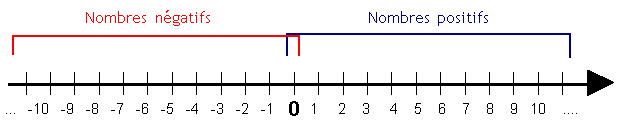
\includegraphics[scale=0.7]{relatifs}
		\end{center}
		
		\item Les nombres positifs et négatifs forment l'ensembles des %\kw{nombres relatifs}.
		
		\item Un nombre relatif est composé d'un \hspace{3cm} (+ ou -) et d'une %\kw{distance à zéro}.
		
		\item Deux \hspace*{5cm} ont la \hspace*{6cm} et des %\kw{signes différents} .
		
	\end{itemize}
\end{mydefs}

%\begin{myrem}
%	0 est le seul nombre à être à la fois positif et négatif.
%\end{myrem}

\begin{myexs}
	\begin{itemize}
		\item $+7$ est un nombre \hspace*{3cm}, sa distance à zéro est %$7$;\\ 
		\begin{center}
			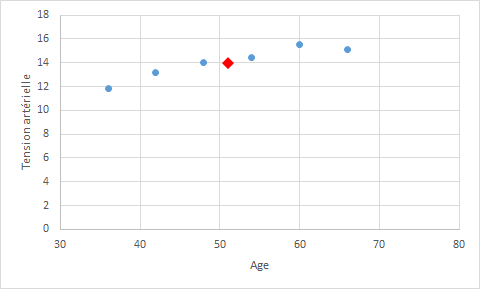
\includegraphics[scale=0.8]{ex1}
		\end{center}
		\item $\num{-4}$ est un nombre \hspace*{3cm}, sa distance à zéro est %$\num{4}$;\\ 
		\begin{center}
			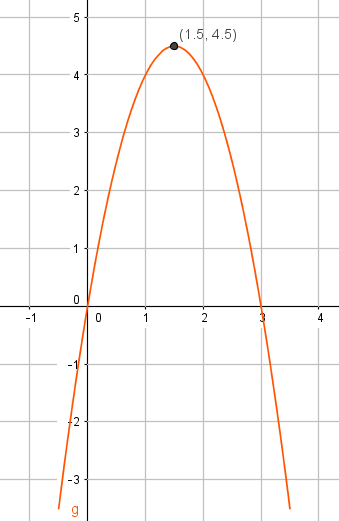
\includegraphics[scale=0.8]{ex2}
		\end{center}
		\item $0$ est %à la fois un nombre positif et négatif.%, sa distance à zéro est 0.
		\item $-10$ et $+10$ sont opposés.
		\begin{center}
			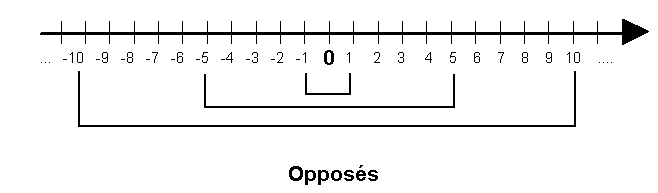
\includegraphics[scale=0.7]{opposes}
		\end{center}
	\end{itemize}
\end{myexs}